%%%%%%%%%%%%%%%%%%%%%%%%%%%%%%
% 	   美赛模板,正文部分		 
%          PAPER.tex         
%%%%%%%%%%%%%%%%%%%%%%%%%%%%%%

%% Reference
%% Abstract
%% Appendice
%% Strength Weakness
\documentclass[12pt]{article}

% 请在此填写控制号、题号和标题,年份不需要填(自动以当前电脑时间年份为准)
\usepackage[1923231]{easymcm}\problem{C}   
\usepackage{palatino} % 这个是COMAP官方杂志采用的字体,如不需要可注释掉,以使用默认字体
\usepackage{subfigure}
\usepackage{float}
\usepackage{IEEEtrantools}
\captionsetup[figure]{font=scriptsize}
\title{\large Modified Lotka-Volterra Model analysing and predicting opioid use}  % 标题
\setlength\parindent{0pt} %default no indent
\newcommand{\upcite}[1]{\textsuperscript{\textsuperscript{\cite{#1}}}}
\renewcommand{\figurename}{Fig.}
% 如您参加的是ICM(即选择了D/E/F题),请使用以下的命令修改Summary Sheet题头
% \renewcommand{\contest}{Interdisciplinary Contest in Modeling (ICM) Summary Sheet}

% 正文开始
\begin{document}
%%%%%%%%%%%%%%%%%%%%%%%%%%%%%%%%%%%%%%%%%
%%            请在此填写摘要            %%
%%%%%%%%%%%%%%%%%%%%%%%%%%%%%%%%%%%%%%%%%
\begin{abstract}\small
A non-SPA-style bathtub cannot be reheated by itself, so the water will get noticeably
cooler and users should add hot water from time to time. Based on the existing Partial
Differential Equation (PDE) technique, we construct time-space based temperature model
which can simulate any common condition. And then propose an optimal strategy
for users to keep the temperature even and close to initial temperature and decrease the
water consumption.

Firstly, we construct the PDE-solving model to simulate the temperature distribution
in the bathtub by analyzing the heat loss and confirming the corresponding parameters.
In this part, we consider two kinds of heat transfer, (water-bathtub heat conduction,
water-air heat convection), and the effect of inflow water on the faucet is shown by the
heat source. So we can confirm the boundary conditions of PDE to carry out the next
step.

Secondly, we do parameter testing by free cooling process to ensure the parameters
are in line with the actual condition. Most of the parameters are applicable, and a few
parameters are fine-tuned to make the model more accurate and practicable.
Thirdly, we confirm the optimal strategy by analyzing and comparing the continuous
and discontinuous flow methods, which vary from the temperature and flux. There are
two feasible methods gained from the analyses, one is continuous 42 $^\circ$C water inflow, the
other is turning on and off the faucet with 42 $^\circ$C inflow for 10 minutes.In addition, we
give two more kinds of methods.

At last, we use our model to determine the extent to which our strategy depends on
the factors of the bathtub, the factors of the user, and a bubble bath additive. And we test
the methods by changing the initial temperature. From those results, we further suggest
the users move less and use more bubble bath additive, and turning on the faucet at the
beginning is also a good choice.
\end{abstract}



%%%%%%%%%%%%%%%%%%%%%%%%%%%%%%%%%%%%%%%%%%
% 如不理解以下部分中各命令的含义,请勿修改! %
%%%%%%%%%%%%%%%%%%%%%%%%%%%%%%%%%%%%%%%%%%

%---------以下生成sheet页----------
% 下面的语句可调整全文行距为标准值的0.6倍,请自行使用
%\renewcommand{\baselinestretch}{0.6}\normalsize
\maketitle  % 生成sheet页
\thispagestyle{empty}   % 不要页眉页脚和页码
\setcounter{page}{-100} % 此命令仅是为了避免页码重复报错,不要在意

%---------以下生成目录----------
\newpage
\tableofcontents
\thispagestyle{empty}   % 不要页眉页脚和页码
\newpage

%---------以下生成正文----------
\setlength\parskip{0.8\baselineskip}  % 调整段间距
\setcounter{page}{1}    % 从正文开始计页码
\pagestyle{fancy}		% 摘要请到ABSTRACT.tex中填写

\section*{Memo}
\addcontentsline{toc}{section}{Memo}
\noindent\rule{\textwidth}{0.8pt}
\textbf{To:} Chief Administrator, NFLIS, DEA \newline
\textbf{From:} Modelers from Team 1923231\newline
\textbf{Subject:} Insights and Results During Modeling\newline
\textbf{Date:} Jan 28, 2019\newline
\noindent\rule{\textwidth}{0.8pt}
\subsubsection*{Intention}
The misuse of opioids has become an national crisis, hence it is urgent to fight against it. We are especially interested in this problem and determined to contribute. Using the dataset provided by NFLIS, we aim to address the insights and recommendations for you.

\subsubsection*{Our Work}
Initially, we use Logistic Regression Model to characterize the trend of opioids use in early stage and identify the maximum number of possible use. This can be used in our second model -- Lotka-Volterra Model when different regions begin to influence each other. It can be used to forecast the use trend in the future. Further, we take socio-economic factors into consideration and find out factors that are decisive for every region.

\subsubsection*{Insights of Dataset}
During we analyze the dataset, we have the following insights:
\begin{itemize}
	\item The influencing factors for different regions differ greatly.
	\item In the short term, controlling the drug use by force in one region may lead to an increase in the neighboring region.
	\item In the long term, educational level and family environment such as marital status have paramount effects on drug use.
\end{itemize}

\subsubsection*{Recommendations}
Based on our research, we have some recommendations for DEA:
\begin{itemize}
	\item Reduce the possibility of making regional policies, take national action instead.
	\item Promote the educational level and family satisfication of the public, which can be achieved by developing the economic and others.
\end{itemize}
\newpage

\section{Introduction}
\subsection{Background}
Opioids, no matter synthetic ones or non-synthetic ones, play an significant role in our daily life. The proper utilization of opioids helps thousands of people get relieved from their pains. However, misuse of them can really destroy the society. Therefore, it is essential and urgent to gain a better understanding of opioids' spread and influencing factors.

Recent years have witnessed the tremendous growth of opioids cases. How this trend will develop remains an national concern. With data of annual drug use and socio-economic factors in five U.S. states over the past few years, we perform data mining and construct a model to figure out the pattern of opioids use and what contributes to it.

\subsection{Problem Statement and Analysis}
The problem is about the opioid crisis in the U.S. society, offering us a set of data ranging from 2010 to 2017. Our main task is to build models that enable us to identify the locations where specific opioid use started and describe the patterns and characteristics of opioid incidents spread. 

First, this is a typical data problem, so we should carefully preprocess the data provided. In the MCM\_NFLIS Data, there are 461 counties belongs to 5 states. For most of the counties, the drug reports are fluctuant, even with large amount of missing data. Besides if we combined all the drug reports of certain state, the start of specific opioid use of one county may be covered up by opioid use of other counties. Therefore, in order to increase the stability of patterns without losing the accuracy, we use the K-means algorithm to combine 461 counties into 10 clusters for our further modeling.

While in the U.S. Census socio-economic data, there are about nearly 600 variables ranging from 2010 to 2017, which is too large to use in the model. We notice that every variable can be classified into certain category by its name, like “HOUSEHOLDS BY TYPE”, “MARITAL STATUS” and so on. It's reasonable to use Entropy Weight Method to combine 596 variables into 15 factors.

Second, in the early development stage of the heroin incidents, we think such incidents can be treated as individual events and the interaction between different states has not yet been formed. So we use the Logistic Model to describe the initial trend of heroin incidents. Through the Logistic Model, we can also get the maximum number of each cluster, which will be used in the next part to determine the threshold levels.

Third, with the spread of incidents, states may start interact with each other and a stable environmental condition for the Logistic Model is no longer met. Therefore, we use the Lotka-Volterra Model to study the spread and characteristics of the reported incidents and forecast the future trend of the heroin incidents. Then we use the Modified Lotka-Volterra Model by adding different factors.

Finally, the Modified Lotka-Volterra Model can provide us both the relationships between clusters and the influence of different factors. By taking all these factors into account, we can identify a possible strategy for countering the opioid crisis and test the effectiveness of this strategy by our model.

\begin{figure}[H]
	\centering
	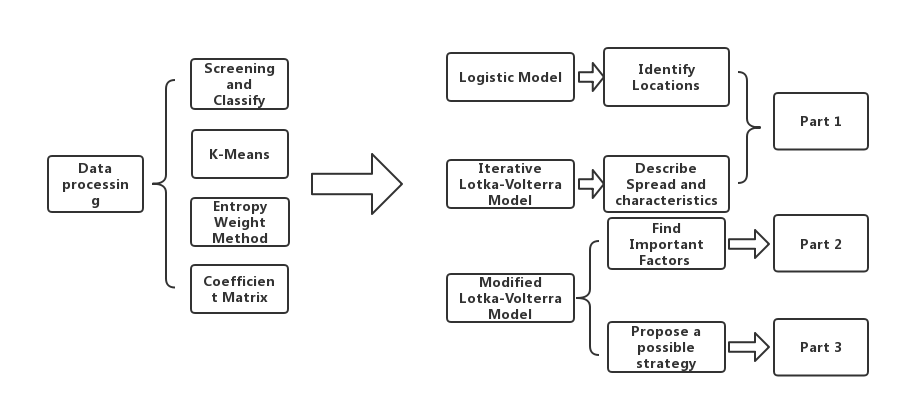
\includegraphics[scale=0.4]{./figures/18.png}
	\caption{Overall Flow Graph}
	\label{Fig18}
\end{figure}

\section{Assumptions and Notations}
\subsection{Assumptions}
Given the lack of necessary data and limitation of our knowledge, we made the following assumptions to help us perform modeling. These assumptions are the premise for our subsequent analysis:
\begin{itemize}
	\item The data after our process are correct and robust for our further analysis.
	\item For the early development stage of the heroin accidents, we assume the incidents growth rate of certain cluster is determined only by itself and the environmental remains stable. So we use the Logistic Model to describe the initial trend of heroin incidents.
	\item The policy of each state will not change in the future. Because policy change will greatly influence the interaction between clusters and the influence of factors, it’s essential for us to assume the policy remain unchanged.
	\item The influence of the factors to heroin incidents remain unchanged and the factors of each clusters grow linearly.
\end{itemize}

\subsection{Notations}
The primary notations used in this paper are listed in Table \ref{tb:notation}.
\begin{table}[!htbp]
\small
\begin{center}
\caption{Notations}
\begin{tabular}{cc}
	\toprule
	\multicolumn{1}{m{3cm}}{\centering Symbol}
	&\multicolumn{1}{m{8cm}}{\centering Definition}\\
	\midrule
	$u_{k}(t)$ &Drug reports of Cluster-k at time t\\
	$ K $ & Upper Bound of Drug Use \\
	$X_{t}$ & Factors calculated by Entropy Weight Method\\
	$a_{k}$ & The natural growth rate of Cluster-k\\
	$b_{jk}$ & The influence factors of Cluster-k to the nature growth rate of Cluster-j\\
	\bottomrule
\end{tabular}\label{tb:notation}
\end{center}
\end{table}

\section{Data Processing}
We are provided with two types of data, the number of drug reports in categories and socio-economic factors. Both of them are specific to counties. The original data contains a lot of redundant and invalid items, which can seriously affect the accuracy and versatility of our model. Thereby, we first apply some data processing techniques before we construct the model.

\subsection{Missing Data Processing}
% In US, each county is assigned a unique five-digit code called FIPS county code. 
In the worksheet about socio-economic factors, there are many cells that contain no valid information at all. We delete columns and rows which contains a lot of useless cells. For other columns and rows, when invalid items appear, we replace it with the average value of the entire sequence.

\subsection{Combine variables into a Socio-economic Factor}
For every year from 2010 to 2016, there are a list of variables about one single socio-economic factor. For instance, factor ANCERSTRY includes estimate, estimate margin of error, percent, etc. Those variables all reflect some information of the target factor in some aspects, hence how to rank their importance matters. 

In information theory, entropy represents the information a sequence contains\upcite{3}. So Entropy Weight Method (EWM), which gives each index a weight according to their entropy, is chosen to measure the significance of each index. Before that, we normalize the data given using the following equation.
\begin{equation}
	y_{i} = \frac{x_{i}-min(x_{i})}{max(x_{i}) - min(x_{i})}
\end{equation}
where $x_{i}$ and $y_{i}$ denotes the original sequence and processed sequence.

We apply EWM in the way addressed as follows (Using ANCERSTRY as an example):
\begin{itemize}
	\item Define Estimate, Estimate margin of error, Percent, Percent margin of error of ANCERSTRY is defined as $y_{j}$ ($y_{1}$ means Estimate...). Compute entropy for $y_{j}$: $ E_{j} = -\frac{\sum p_{i}lnp_{i}}{ln(n)}$, where $p_{i}=\frac{y_{ji}}{\sum_{i} y_{ji}}$, $E_{j}$ represents the entropy for each index.
	\item Compute weight for Estimate, Estimate margin of error, Percent, Percent margin of error of ANCERSTRY: $ W_{j} = \frac{E_{j}}{\sum E_{j}}$, where $W_{j}$ represents the weight for each index.
	\item Combine variables using the weight: $X_{i} = \sum_{j} W_{j} * y_{ji}$
\end{itemize}
So far, we have combined several variables of a factor into one $X$, and the same can be done to other factors. The newly generated sequence will be reserved for further analysis.

\subsection{Cluster Counties of Five States}
Since we have detailed number of drug reports, it is not hard to fit a curve to observe the trend of opioid use for each state and for each county. However, we consider this method inappropriate. On the one hand, the sample for only one county is normally fluctuating irregularly, i.e. drug reports of heroin in ACCOMACK, VA was 2, 38, 6 during 2012-2014. It is unnecessary and meaningless to bulid a model when facing such fluctuation. On the other hand, given the large number of all kinds of opioids, even one type change significantly, it is not obvious when viewed as the level of the whole state.

Considering that state and county are not suitable for our research, a unit in between is introduced. We put counties on a two-dimensional plane and regard them as nodes. Then, k-means clustering method\upcite{1}, which aims to partion nodes into $k$ clusters minimizing the within-cluster sum of squares, was performed. In our case, we take $k = 10$. The distance of two counties can be computed with their latitude and longtitude retrieved from U.S. Census Bureau\upcite{2}. The clusters we derived are labeled as Cluster-1, Cluster-2, ..., Cluster-10.
\begin{figure}[H]
	\centering
	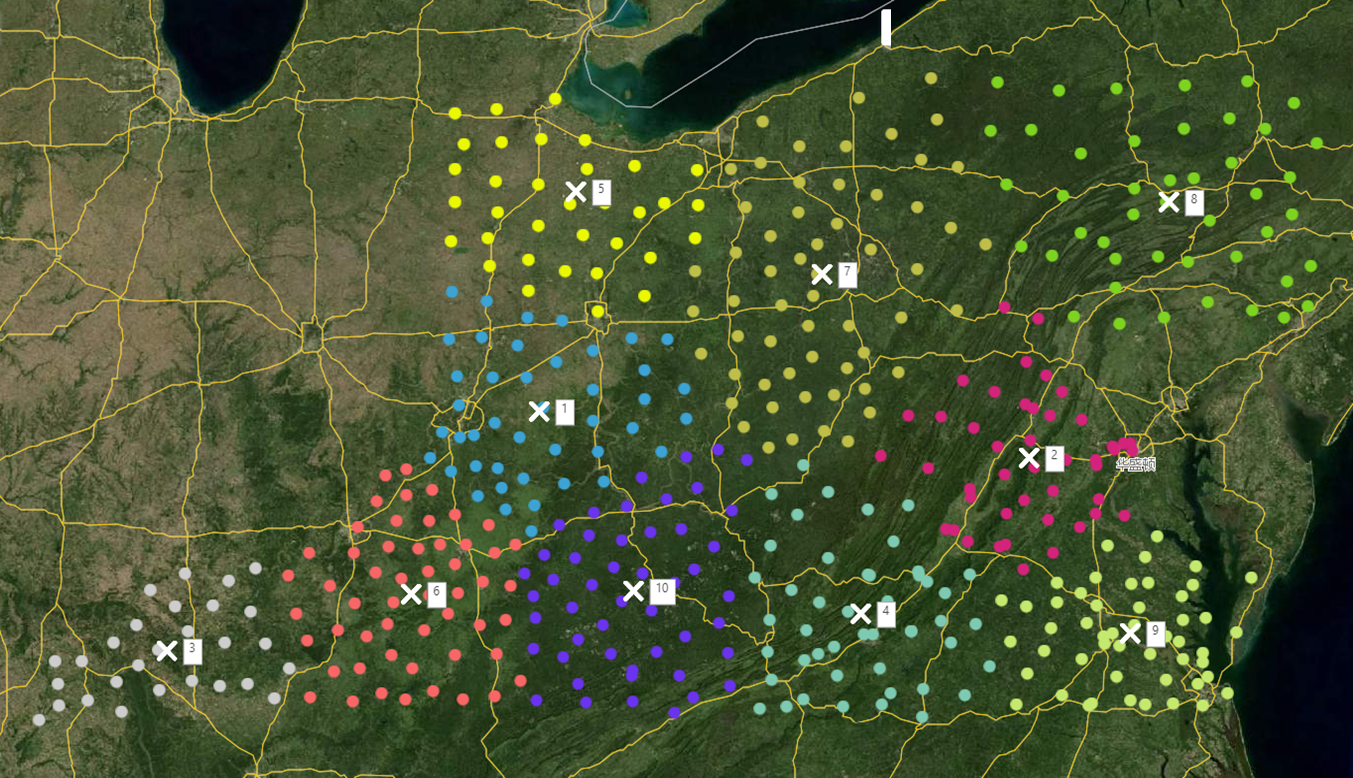
\includegraphics[scale=0.3]{./figures/0.png}
	\caption{Clusters got after k-means, points with the same color belong to one cluster}
	\label{Fig0}
\end{figure}

\subsection{Data Screening -- Drug Classification}
In order to describe the dissemination and characteristics of the synthetic opioids and heroin spread sperately, we need to screen the information in MCM\_NFLIS\_Data.xlsx. By consulting Wikipedia, DrugBank\upcite{4} and other websites, provided drugs are roughly classified into synthetic opioids, semi-synthetic opioids, and natural ingredients(Table \ref{opioid kind}). In view of the topic requirements, we excluded the natural ingredients and drugs other than heroin in semi-synthetic opioids, leaving the drug reports of heroin and synthetic opioids only. As for the synthetic opioid, we find that many drugs have been used in small amounts over the years compared to those used in large numbers. And some drugs only start to appear in the past two years, so we can just ignore them. Finally, we leave about 15 kinds of synthetic drugs that have appeared since 2010 for further research.
\begin{table}[H]
	\small
	\centering
	\caption{Opioids and Their Kind}
	\begin{tabular}{c|l}
	\hline
	Kind & Specific Opioids\\
	\hline
	Natural Ingredients	& Codeine, Morphine, Opium \\
	\hline
	Semi-synthetic Opioids & DIhydrocodeine, Heroine, Opiates, Oxycodone, Oxymorphone\\
	\hline
	Synthetic Opioids &  ANPP, Buprenophine, Butorphanol, Fentanyl, Meperidine, Methorphan\\
	\hline
	\end{tabular}
	\label{opioid kind}
\end{table}

\section{Model Construction}
\subsection{Identify Locations using Logistic Model}
\subsubsection{Model Establishment}
With the k-means cluster analysis, we acquire data about the synthetic opioid and heroin events in ten clusters. It is clear to identify that the drug use levels in most areas are increasing. If drug use continues to grow at such speed, it will bring about numerous negative effects to the society when it exceeds an certain level, as mentioned in the Problem Background. Therefore, government’s relevant departments, including the Drug Enforcement Administration(DEA), will take corresponding measures to control the growing trend of drug use. However, when consumptions reach a high level, the growing rate in usage will reduce. And it is gradually increasing when consumptions are low.

The regular drug-use pattern is identical to the Logistic model of population growth, in which the natural growth rate of the population will be limited by the population. Similarly, the drug-use will be limited by many restrictions including social factors such as government control and natural factors such as population growth. Assuming that drug-use level could be affected by these factors and thus having a ceiling, it can be considered that the growth trend of synthetic opioid and heroin events are subordinated to the Logistic model. Here’s the Logistic model:
\begin{equation}
	\begin{split}
	\frac{du(t)}{dt} = r&(1-\frac{u(t)}{K})u(t) \label{logistic}\\
	u(t_{0}) &= u_{0}
	\end{split}
\end{equation}

where $u(t)$ represents the drug-use amount time $t$, $K$ represents the upper bound of the drug-use level and $r$ means an influence factor of the drug-use amount. The model can be understood that there is no strict control and the drug is attractive in the early time, which results in the quickly increase of the drug use. As some departments begin to pay attention to this phenomenon and implement policies to control it, the growth rate of drug use begins to decrease. When the drug-use level is close to the allowable upper bound, $\frac{(1-Q)}{K} \approx 0$ . At this point, the drug-use level will no longer increase. Considering that our model is discrete in time,  we replace $\frac{du(t)}{dt}$ with $N(t+1)-u(t)$.

The following equations gives the solution of logistic regression (Equation (\ref{logistic})).
\begin{gather}
	u(t)=\frac{K}{1+Ce^{-r(t-t_{0})}} \\
	C=\frac{K-u_{0}}{u_{0}} 
\end{gather}
The above mathematical formulas and model can be established by programing. We utilize the data of ten clusters to buildthe model and acquire the logistic regressing curves.

\subsubsection{Model Application and Problems Solving}
In order to test the effectiveness of our model, we first put the total drug reports into the model for regressing and fitting, and get the following results. From the above clusters mentioned, the drug-use level in some areas is decreasing or fluctuating, we find three unsuitable clusters(Cluster-4, Cluster-5, Cluster-10) and the Fig. \ref{Fig.1} can show that those data are not suitable in this model. Therefore we cannot use the Logistic population growth model to perform regression of these areas’ drug reports. That is to say, other models may be needed for their prediction, which is not considered currently.

\begin{figure}[H]
	\centering %图片全局居中
	%并排几个图,就要写几个minipage
	\begin{minipage}[b]{0.45\textwidth} %所有minipage宽度之和要小于1,否则会自动变成竖排
		\centering %图片局部居中
		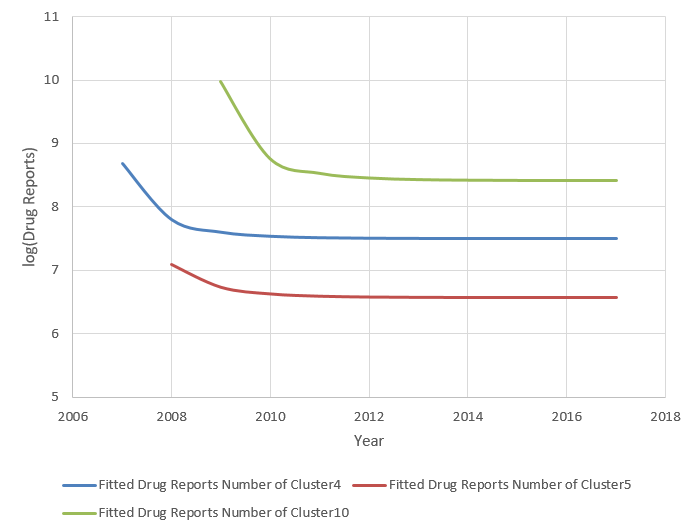
\includegraphics[scale=0.45]{./figures/1.png} %此时的图片宽度比例是相对于这个minipage的,不是全局
		\caption{Total Drug Reports Curves of Unsuitable Clusters}
		\label{Fig.1}
	\end{minipage}
	\begin{minipage}[b]{0.45\textwidth} %所有minipage宽度之和要小于1,否则会自动变成竖排
		\centering %图片局部居中
		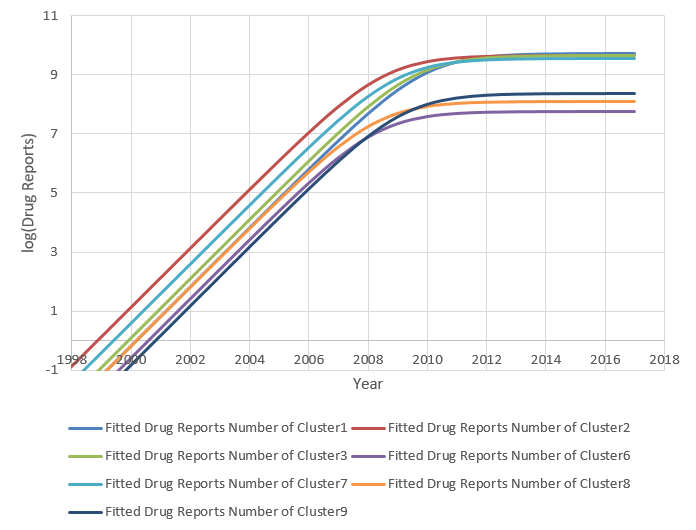
\includegraphics[scale=0.5]{./figures/2.png}%此时的图片宽度比例是相对于这个minipage的,不是全局
		\caption{Total Drug Reports Curves of Suitable Clusters}
		\label{Fig.2}
	\end{minipage}
\end{figure}

% \begin{figure}[H]
% 	\centering
% 	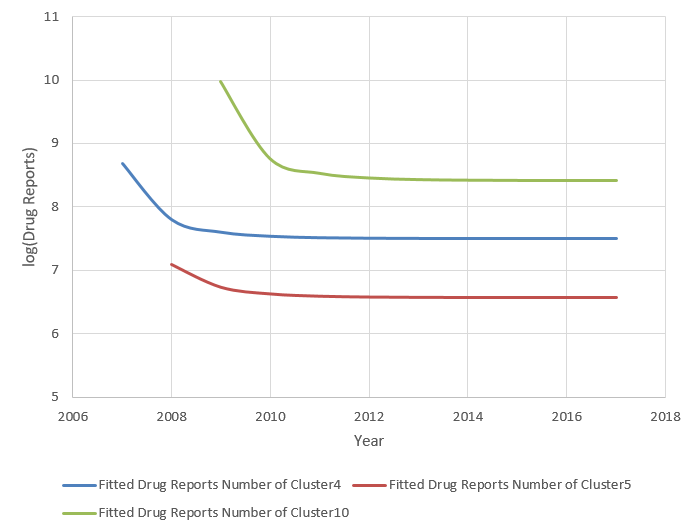
\includegraphics[scale=0.6]{./figures/1.png}
% 	\caption{Total Drug Reports Curves of Unsuitable Clusters}
% 	\label{Fig.1}
% \end{figure}

According to fitted curves of the remaining data, we obtain the curves of drug-use level for 20 years from 2000 to present. Then, we look for intersections of every curve and the time axis. Fig. \ref{Fig.2} describes most clusters’ characteristics of total drug use.

We can clearly see that Cluster-2, where drug cases have started since 1999, is earlier than any other six clusters and this is exactly our target to find in specific opioids in most clusters. Consulting the map of U.S., we know that Cluster-2 represents east of West Virginia area.

Therefore, we further make use of this model to analyze the usage of heroin and synthetic opioids screened in data screening and acquire the following results.

\begin{figure}[H]
	\centering %图片全局居中
	%并排几个图,就要写几个minipage
	\begin{minipage}[b]{0.48\textwidth} %所有minipage宽度之和要小于1,否则会自动变成竖排
		\centering %图片局部居中
		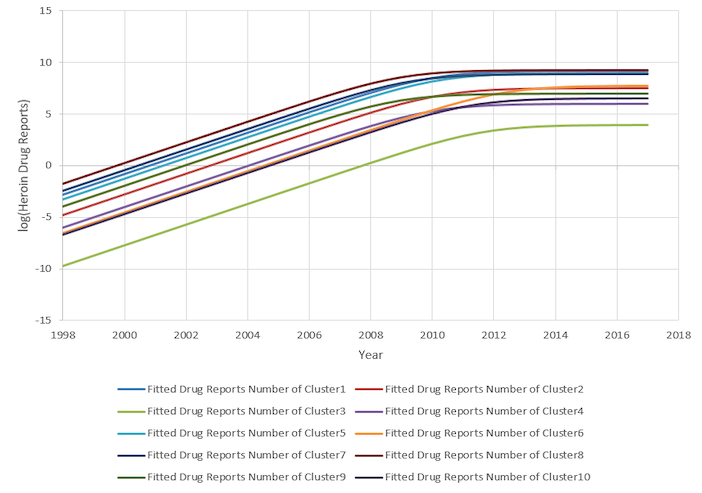
\includegraphics[scale=0.45]{./figures/3.png} %此时的图片宽度比例是相对于这个minipage的,不是全局
		\caption{Drug Reports for Heroin}
		\label{Fig.3}
	\end{minipage}
	\begin{minipage}[b]{0.48\textwidth} %所有minipage宽度之和要小于1,否则会自动变成竖排
		\centering %图片局部居中
		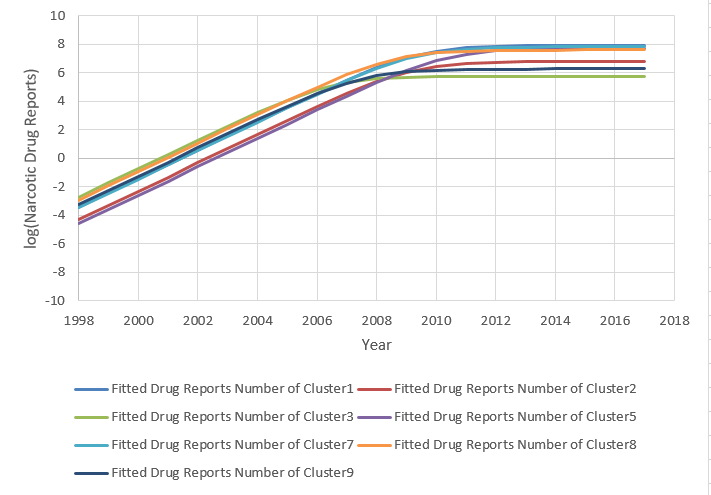
\includegraphics[scale=0.6]{./figures/4.png}%此时的图片宽度比例是相对于这个minipage的,不是全局
		\caption{Drug Reports for Syntheic Opioids}
		\label{Fig.4}
	\end{minipage}
\end{figure}

As we can see from Fig. \ref{Fig.3}, the Cluster-8(Pennsylvania) in the ten clusters has already started using heroin drugs before 2000. It can be considered that counties which belonging to Cluster-8 could be the locations where heroin started to appear and use.

In Fig. \ref{Fig.4}, it can be seen that Cluster-1, 3, 7, 8, and 9 all started using drugs around 2001. Because the time accuracy is not particularly precise, they may all be the areas where synthetic opioids were used earlier. According to our model, we believe that the Kentucky represented by Cluster-3 is the area where the synthetic opioids use have started earlier.

What’s more, we use the logistic discrete equation to solve the coefficients of the regression, and obtain the maximum tolerance of drug-use in each region based on this model. Results presented presented in the following table will continue to be used in subsequent models.
\begin{table}[H]
	\centering
	\caption{Maximum Tolerance(MT) for Clusters}
	\begin{tabular}
	{cccccc}
	\toprule[1pt]
	Cluster	& 1 & 2 & 3 & 4 &5 \\
	MT	& 44101 & 22261 & 1909 & 602 & 2840\\
	\midrule
	Cluster	& 6 & 7 &  8 & 9 & 10 \\
	MT & 2840 & 19022 & 3330 & 4318 & 6084\\
	\bottomrule[1pt]
	\end{tabular}
\end{table}

\subsection{Describing the spread and characteristics using Iterative Lotka-Volterra Model}
In the last section 4.1, we construct Logistic Model to identify the possible locations where specific opioid use might have started. However, as the number of drug reports approaches the carrying capacity $u_{max}$, the Logistic Model become smooth and can’t provide more information about the changing trends. Therefore, in this section, we modify the dynamic Lotka-Volterra equations to model the interactions between different clusters.
	
The Lotka-Volterra equations are known as the predator-prey equations in a biological system of two (or more) species. In fact, the Lotka-Volterra equations can describe not only the predation relationships between species, but also the competition, parasitism even mutualism relationships. And we think the spread of the reported synthetic opioid and heroin incidents may have a mixed features, which meets the application conditions.

For simplification, let $S_{1}$ and $S_{2}$ denote, respectively, Species 1 and Species 2. Let $u_{1}(t)$ and $u_{2}(t)$ denote, respectively, the measurement of $S_{1}$ and $S_{2}$ at time t. Let $a_{1}$ and $a_{2}$ denote the natural growth fate of $S_{1}$ and $S_{2}$, and $b_{1}$ and $b_{2}$, respectively, the influence factor of $S_{1}$ to the natural growth rate of $S_{1}$ and $S_{2}$. Similarly, here goes the $c_{1}$ and $c_{2}$. The Lotka-Volterra equations are non-linear, first-order differential equations defined as follows:
\begin{gather}
	u'_{1}(t) = u_{1}(t)(a_{1} + b_{1}u_{1}(t) + c_{1}u_{2}(t)) \label{equ41}\\
	u'_{2}(t) = u_{2}(t)(a_{2} + b_{2}u_{2}(t) + c_{2}u_{2}(t))
\end{gather}

Next, we extend and apply the above equations to model interactions between the 10 clusters. Let $u_{k}(t)$ denote the Cluster-k, where k = 1,2,…,10. Let $a_{k}$ denote the change rate of Cluster-k itself, and $b_{kj}$ denote the influence of Cluster-j to Cluster-k. The equations can be written as
\begin{equation}
	\begin{split}
	\frac{du_{k}(t)}{dt} &= u_{k}(t)(a_{k} + \sum_{j=1}^{9}b_{jk}u_{k}(t)) \\
	k &= 1,2,..,9
	\end{split}
\end{equation}

\begin{equation}
	\begin{pmatrix}
		\frac{du_{1}(t)}{dt} \\
		\frac{du_{2}(t)}{dt} \\
		\vdots \\
		\frac{du_{9}(t)}{dt}	
	\end{pmatrix}
	=
	\begin{pmatrix}
		u_{1}(t) \\
		u_{2}(t) \\
		\vdots \\
		u_{9}(t)
	\end{pmatrix}
	\otimes
	\begin{pmatrix}
		a_{1} & b_{11} & \ldots & b_{19}\\
		\vdots & \vdots & \ddots & \vdots\\
		a_{9} & b_{91} & \ldots & b_{99}
	\end{pmatrix}
	\ast
	\begin{pmatrix}
		1 \\
		u_{1}(t) \\
		u_{2}(t) \\
		\vdots \\
		u_{9}(t)
	\end{pmatrix}
\end{equation}

For the ease of calculation and prediction, we modify the equation as follows. Let $\bm{\bar U(t)}$ denote the vector $\bm{[du_{k}(t)/dt]^{T}_{1*n}}$  , $\bm{U(t)}$ denote the vector $\bm{[u_{k}(t)]^{T}_{1*n}}$  , $\bm{A}$ denote the matrix $\bm{[\bar a | {\bar B}]}$ where $\bm{{\bar a}=[a_{k}]^T_{1*n}}$  , $\bm{{\bar B}=[b_{kj}]_{n*n}}$.
\begin{equation}
	\bm {{\bar U(t)}=U(t)\otimes A \times [1 | U(t)^{T}]^{T}}
\end{equation}

We notice the time parameter is discrete. In order to make the equation iterated, we transformed equations as follows:
\begin{equation}
	\begin{pmatrix}
		\frac{1}{u_{1}(t)}\frac{du_{1}(t+1)}{dt} \\
		\frac{2}{u_{2}(t)}\frac{du_{2}(t+1)}{dt} \\
		\vdots \\
		\frac{3}{u_{3}(t)}\frac{du_{3}(t+1)}{dt}	
	\end{pmatrix}
	=
	\begin{pmatrix}
		\frac{u_{1}(t+1)}{u_{1}(t)} - 1 \\
		\frac{u_{2}(t+1)}{u_{2}(t)} - 1 \\
		\vdots \\
		\frac{u_{9}(t+1)}{u_{9}(t)} - 1
	\end{pmatrix}
	=
	\begin{pmatrix}
		a_{1} & b_{11} & \ldots & b_{19} \\
		\vdots & \vdots & \ddots & \vdots \\
		a_{9} & b_{91} & \ldots & b_{99}
	\end{pmatrix}
	\ast
	\begin{pmatrix}
		1 \\
		u_{1}(t) \\
		u_{2}(t) \\
		\vdots \\
		u_{9}(t)
	\end{pmatrix}
\end{equation}

\begin{equation}
	\begin{pmatrix}
		\frac{u_{1}(t+1)}{u_{1}(t)} \\
		\frac{u_{2}(t+1)}{u_{2}(t)} \\
		\vdots \\
		\frac{u_{9}(t+1)}{u_{9}(t)} \\
	\end{pmatrix}
	=
	\begin{pmatrix}
		a_{1} & b_{11} & \ldots & b_{19} \\
		\vdots & \vdots & \ddots & \vdots \\
		a_{9} & b_{91} & \ldots & b_{99}
	\end{pmatrix}
	\ast
	\begin{pmatrix}
		1 \\
		u_{1}(t) \\
		u_{2}(t) \\
		\vdots \\
		u_{9}(t)
	\end{pmatrix}
	+
	\begin{pmatrix}
		1 \\
		1 \\
		\vdots \\
		1
	\end{pmatrix}
\end{equation}

\begin{equation}
	\begin{pmatrix}
		u_{1}(t+1) \\
		u_{2}(t+1)\\
		\vdots \\
		u_{9}(t+1) \\
	\end{pmatrix}
	=
	\begin{pmatrix}
		u_{1}(t) \\
		u_{2}(t) \\
		\vdots \\
		u_{9}(t)
	\end{pmatrix}
	\otimes 
	\left \{
	\begin{pmatrix}
		a_{1} & b_{11} & \ldots & b_{19} \\
		\vdots & \vdots & \ddots & \vdots \\
		a_{9} & b_{91} & \ldots & b_{99}
	\end{pmatrix}	
	\ast
	\begin{pmatrix}
		1 \\
		u_{1}(t) \\
		u_{2}(t) \\
		\vdots \\
		u_{9}(t)
	\end{pmatrix}
	+
	\begin{pmatrix}
		1 \\
		1 \\
		\vdots \\
		1
	\end{pmatrix}
	\right \}
\end{equation}

And we get the final iterative equation as follows:
\begin{equation}
	\bm{U(t+1) = U(t)} \otimes \{\bm{A * [1 | U(t)}^{T}]^{T} + 9 * [1]\} = \bm{g(U(t))}
\end{equation}

In order to get the iterative matrix $\bm{A}$, we use the least square method to estimate. For Cluster-i, the vector $[a_{i}, b_{i1}, ..., b_{i9}]$ has 10 parameters, while we only have 8 equations ranging from 2010 to 2017, which can’t meet the condition of least square $n > k$ . Therefore, we use the interpolation method to increase sample points. For simplicity, we take the median of any two adjacent sample points as the interpolation value.

\begin{equation}
	\bm{U}(\bm{t}+\frac{1}{2}) = \cfrac{\bm{U}(\bm{t}+1) + \bm{U}(\bm{t})}{2}
\end{equation}

After implementing the above mathematical model by programming, we obtain the coefficient matrix of regression equation, which represents the effects of clusters self-influence and mutual influence. According to the positive or negative values of the matrix, we can conclude the spread feature of the drug usage over time. 

The positive coefficient value indicates the influence is to promote the drug-use level, contrary to the negative value which represents the impact of restricting growth. As distance factor has an effect on regional spread, attention is paid to the propagation between adjacent clusters regardless of long distance. So we have the following relationship network figure, where the solid line indicates that the effect is positive and the dotted line indicates that the effect is negative.

\begin{figure}[H]
	\centering
	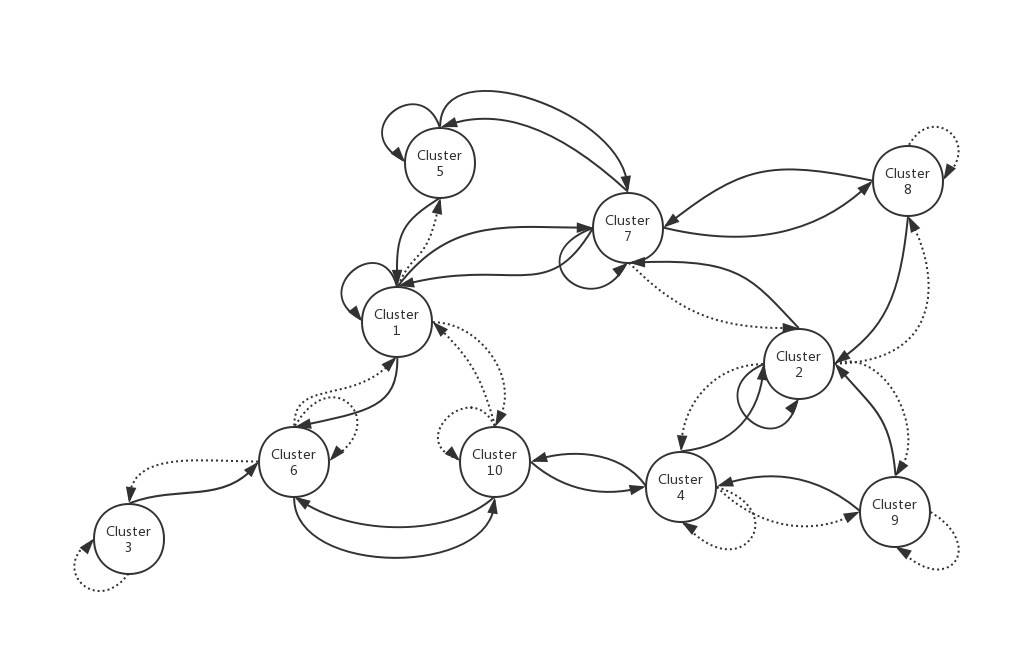
\includegraphics[scale=0.45]{./figures/15.png}
	\small
	\begin{tabular}{rr}
		$\dashrightarrow$ & Negative Effect \\
		$\longrightarrow$ & Positive Effect
	\end{tabular}
	\caption{Clusters' Self-influence and Mutual Influence}
	\label{Fig15}
\end{figure}

According to the logistic model, we have obtained tolerances for drug-use levels in each region, which we approximately consider as the drug threshold level for each region, making an analogy with the maximum environmental capacity in biology. If drug usage exceeds the threshold level, the drug use in this region might become uncontrollable thus resulting in an unprecedented social crisis.

\begin{figure}[H]
	\centering
	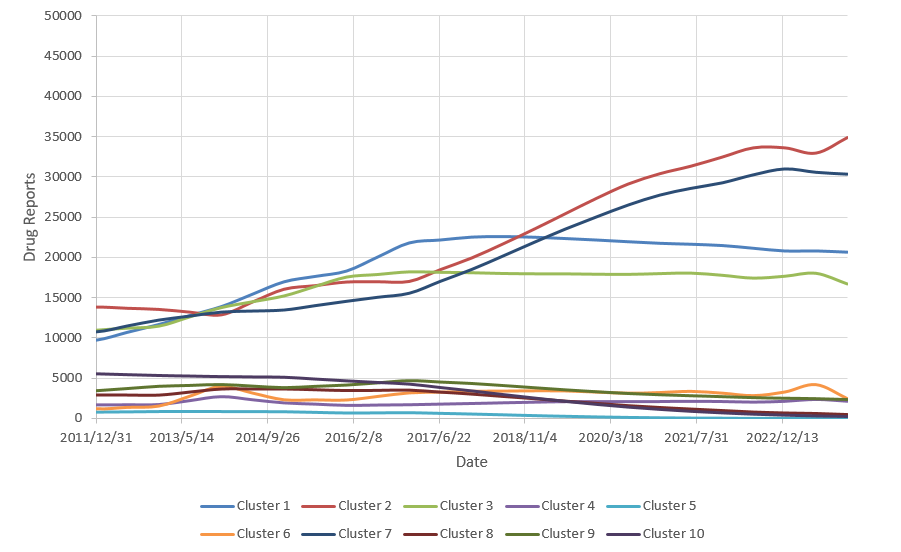
\includegraphics[scale=0.7]{./figures/5.png}
	\caption{Trend of the Next 5 Years}
	\label{Fig5}
\end{figure}

In the above figure, we know that the number of drug use in some areas is decreasing annually or being stable at a relatively low value. So it can be considered that drug usage will not exceed its threshold level in the next few years, and the government does not need to be concerned about these areas, hence we no longer make their curves. Now we focus on clusters with clearly upward drug-use trends. The first goal is to find the intersection of the drug threshold level and the rising curve in order to make a judgement on whether government should take actions. The following figures clearly demonstrates what has been mentioned.

We can see that both Cluster-2 and Cluster-7, which represent east of West Virginia and part of Pennsylvania, exceed the drug threshold levels. Cluster-2 will reach the threshold level 2018, which indicates that local government should take measures as much quickly as possible. And Cluster-7 will reach the threshold a few years later, around 2021. Also, it shows that the rising trend still maintains for the following years. So it can be considered that drug use may be uncontrolled in these two regions when the levels are exceeded. Thus, it is urgent for the government to adopt effective measures in advance.

\begin{figure}[H]
	\centering %图片全局居中
	%并排几个图,就要写几个minipage
	\begin{minipage}[b]{0.48\textwidth} %所有minipage宽度之和要小于1,否则会自动变成竖排
		\centering %图片局部居中
		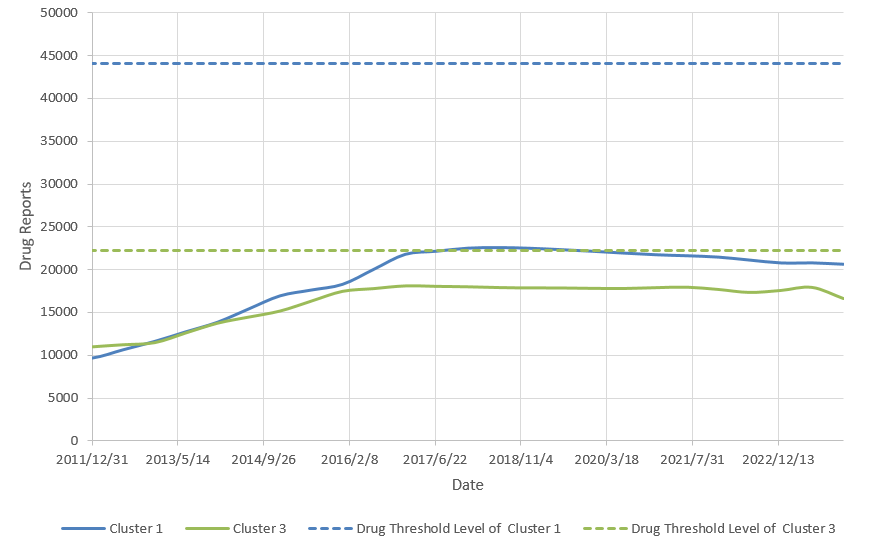
\includegraphics[scale=0.45]{./figures/6.png} %此时的图片宽度比例是相对于这个minipage的,不是全局
		\caption{Threshold levesl of Cluster-1 and Cluster-3}
		\label{Fig6}
	\end{minipage}
	\begin{minipage}[b]{0.48\textwidth} %所有minipage宽度之和要小于1,否则会自动变成竖排
		\centering %图片局部居中
		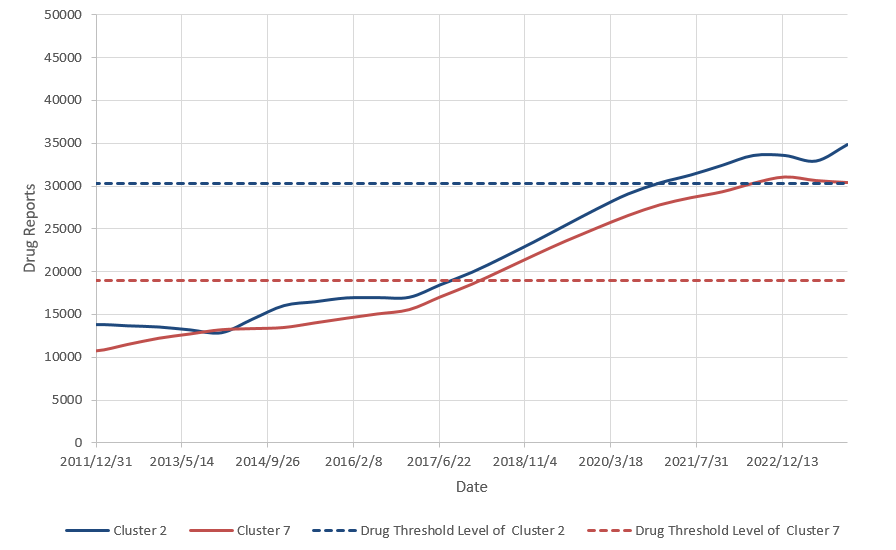
\includegraphics[scale=0.45]{./figures/7.png}%此时的图片宽度比例是相对于这个minipage的,不是全局
		\caption{Threshold Levels of Cluster-2 and Cluster-7}
		\label{Fig7}
	\end{minipage}
\end{figure}


However, the Modified Lotka-Volterra Model we construct is an unstable differential equations. As time goes on, the differential equations system show chaotic phenomena. Every 20 years, all the values of 10 clusters fluctuate severely and then suddenly converge to 0. Fig. \ref{Fig8} depicts the trend of opioid and heroin incidents in the 10 clusters for the next 50 years.
\begin{figure}[H]
	\centering
	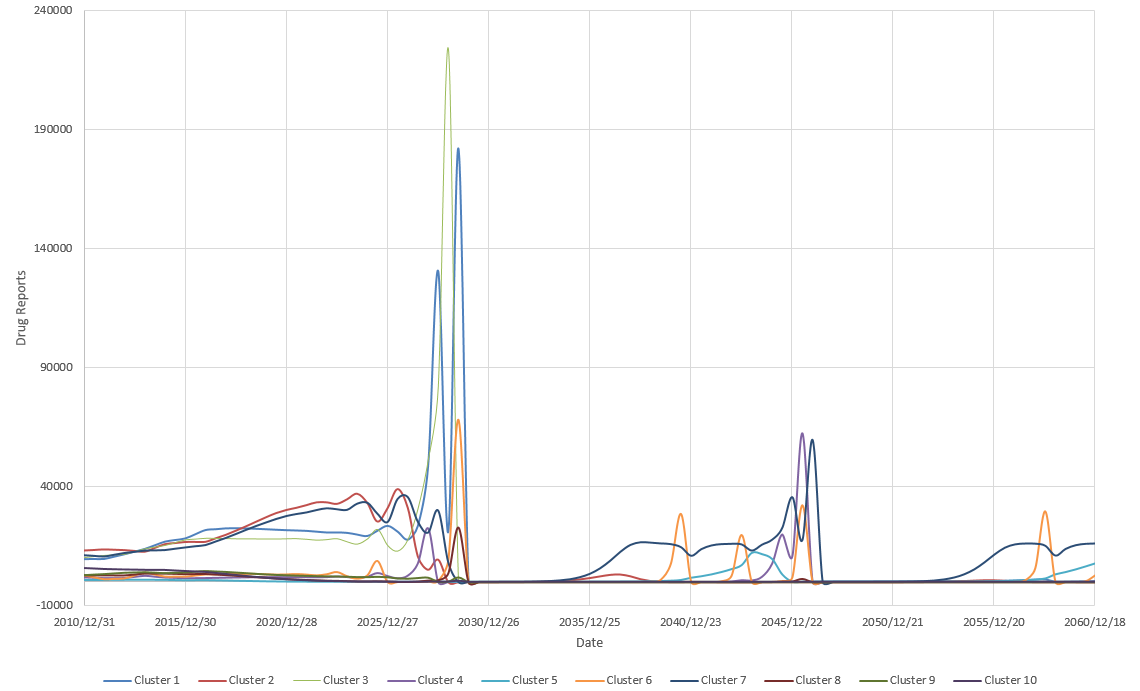
\includegraphics[scale=0.6]{./figures/8.png}
	\caption{Trend of the Next 50 Years}
	\label{Fig8}
\end{figure}

The reasons for the model failure are as follows:
\begin{enumerate}
	\item We use the least square method to estimate the iterative matrix A by samples from 2010 to 2017. However, in the reality, the interactions between different clusters may change with time. \item The patterns and characteristics we derive from samples may continue only for s short time.
	For Equation \ref{equ41}, we set the right-hand side of the system to 0, to get 4 equilibrium points
\end{enumerate}
\begin{gather*}
	A_{1}(0, 0) \\
	A_{2}(0, \frac{c_{1}a_{2}-a_{1}c_{2}}{b_{1}c_{2}-c_{1}b_{2}}) \\
	A_{3}(\frac{b_{1}a_{2} - a_{1}b_{2}}{c_{1}b_{2}-b_{1}c_{2}}, 0) \\
	A_{4}(\frac{b_{1}a_{2} - a_{1}b_{2}}{c_{1}b_{2}-b_{1}c_{2}}, \frac{c_{1}a_{2}-a_{1}c_{2}}{b_{1}c_{2}-c_{1}b_{2}}) 
\end{gather*}

The first three equilibrium points contain the coordinate 0, which contrasts the reality that each species shouldn't extinct. The reasonable equilibrium point $A_{4}$ should meet the conditions:
\begin{gather*}
	\left \vert 
	\begin{matrix}
		a_{1} & a_{2} \\
		c_{1} & c_{2} 
	\end{matrix}
	\right \vert
	\ast
	\left \vert
	\begin{matrix}
		c_{1} & c_{2} \\
		b_{1} & b_{2}
	\end{matrix}
	\right \vert
	> 0 \\
	\left \vert 
	\begin{matrix}
		a_{1} & a_{2} \\
		b_{1} & b_{2} 
	\end{matrix}
	\right \vert
	\ast
	\left \vert
	\begin{matrix}
		b_{1} & b_{2} \\
		c_{1} & c_{2}
	\end{matrix}
	\right \vert
	> 0
\end{gather*}

The matrix $\bar B$ may not satisfy the corresponding conditions.

\subsection{Considering Factors Using Modified Iterative Lotka-Volterra Model}
In the last section, we build the Iterative Lotka-Volterra Model(LVM) to research the interactions between different clusters. However, the LVM can only be applied in a short range of time. In this section, we modify the LVM by adding attribute characters from the U.S. Census socio-economic data.

The U.S. Census socio-economic data has nearly 500 more variables ranging from 2010 to 2016, which is too large to use. In the data process section, we use entropy weight method to further classify variables into 15 factors. The time series of 15 factors in Cluster 1 are listed as follows.

\begin{figure}[H]
	\centering %图片全局居中
	%并排几个图,就要写几个minipage
	\begin{minipage}[b]{0.48\textwidth} %所有minipage宽度之和要小于1,否则会自动变成竖排
		\centering %图片局部居中
		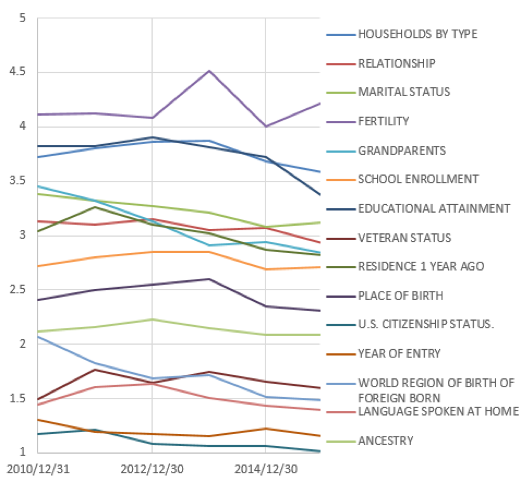
\includegraphics[scale=0.8]{./figures/9.png} %此时的图片宽度比例是相对于这个minipage的,不是全局
		\caption{}
		\label{Fig9}
	\end{minipage}
	\begin{minipage}[b]{0.48\textwidth} %所有minipage宽度之和要小于1,否则会自动变成竖排
		\centering %图片局部居中
		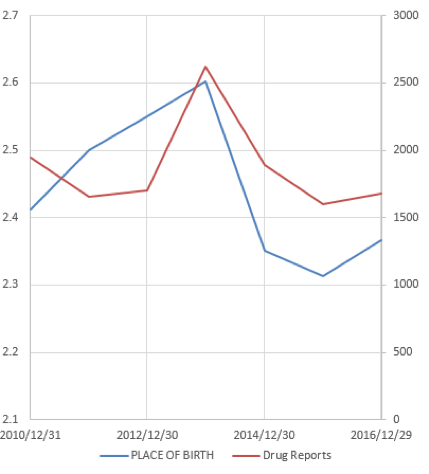
\includegraphics[scale=0.8]{./figures/10.png}%此时的图片宽度比例是相对于这个minipage的,不是全局
		\caption{}
		\label{Fig10}
	\end{minipage}
\end{figure}

As we can see from Fig. \ref{Fig9}, part of those factors are strongly correlated. So certain factors can provide as much information as we need in the model construction. By further process, we find factors 'PLACE OF BIRTH' of Cluster-1 has a similar trend with the Drug Reports of Cluster-1. These findings inspire us that certain factors may help to forecast the trend of Drug Reports. In order to select the best factors to forecast, we calculator the correlation coefficient between every 15 factors and every 10 clusters. The results are put in the Appendix.

Fig. \ref{Fig11} demonstrates the major influential factors. We observe that the influencing factors differ by regions, based on the locations of five states and ten clusters in the map. \ref{Fig11}. So we categorize these influencing factors on a geographical basis, which are presented in \ref{Fig11}.

It is obvious that immigration plays a decisive role in Cluster-2, 8, and 9 near the East Coast. This is not difficult to understand, because many immigrants started locating in the east coast of the United States ever since Columbus discovered the Americas. The immigration culture and degree also determine their preference and use of drugs to some extent. At the same time, the drug-use level in the east of West Virginia area is related to veterans, which can be speculated in the light of the fact that military power concentrates in its vicinity - Washington, DC. 

The main influence factor in the central region is the level of education. Since there are various institutions of high level in these regions (Cluster-1, 5, 7, 10), we can conclude that education is also closely related to drug use. As forwestern regions of the five states, family composition could be the main reason. Based on common knowledge, there is a certain relationship between drug crime, family background and growing environment, the result is convincing.

\begin{figure}[H]
	\centering
	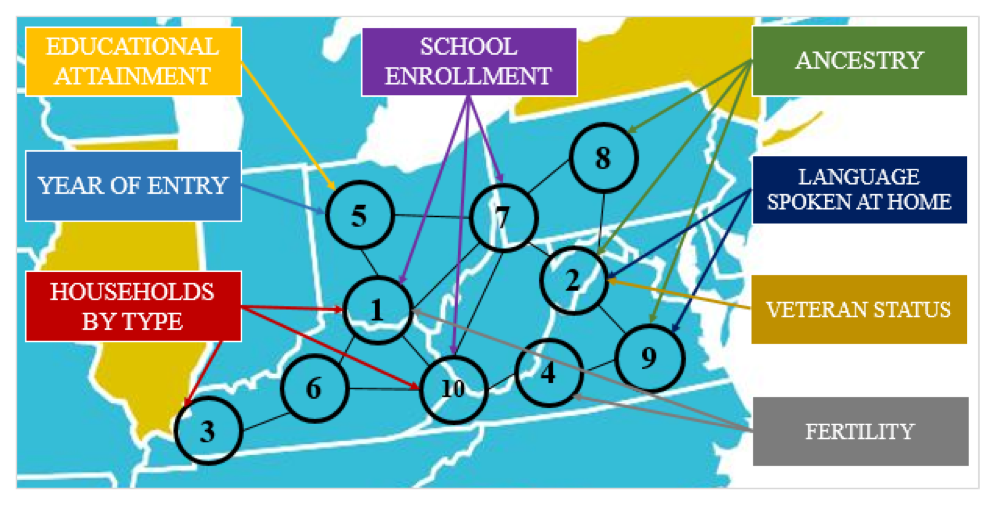
\includegraphics[scale=0.7]{./figures/11.png}
	\caption{Major Influential Factors}
	\label{Fig11}
\end{figure}

Since the Iterative Lotka-Volterra Model doesn’t take the attribute into account, we can modify the model by adding attribute characters from socio-economic factors. For each Cluster, we select the factors most correlated to drug reports (including positive and negative correlation coefficient). And build linear regression model to calculate the change rate of $u_k(t)$ as follows:

\begin{equation}
	\begin{aligned}
		\frac{du_{k}(t)}{dt} &= a + bX_{t}^{k} \\
		&=h(X_{t}^{k}) \\
		k &= 1,2,...,9
	\end{aligned}
	\label{4.7}
\end{equation}

In the LVM, we calculate the change rate of $u_{k}(t)$ by
\begin{equation}
	\begin{aligned}
	\frac{du_{k}(t)}{dt} &= u_{k}(t-1)(a_{k} + \sum_{j=1}^{9}b_{kj}u_{k}(t-1)) \\
	&=f(u_{k}(t-1))
	\end{aligned}
	\label{4.8}
\end{equation}
By formula \ref{4.7}, we get the change rate of $u_k(t)$ by using the attributes of Cluster-k. By formula \ref{4.8}, we get the change rate of $u_k(t)$ by spreading the interactions between different Clusters. To combine both of the influences, we modify the change rate of $u_k (t)$ by taking the weighted average of two results.

\begin{equation}
	\frac{du_{k}(t)}{dt} = \lambda(t)h(X_{t}^{k}) + (1-\lambda(t))f(u_{k}(t-1))
\end{equation}

Because in the short run, the interactions among different clusters remain stable. While in the long run, the macro attributes are more reliable to forecast. Hence the weighted parameter $\lambda(t)$ should satisfy the following properties. 
\begin{equation}
	\lambda(t) \in (0, 1) \lambda'(t) > 0
\end{equation}
where $\lambda(t) = \frac{ln(t)}{1+ln(t)}$.

By calculating, we get the next 50 years of drug reports in different clusters. 
\begin{figure}[H]
	\centering
	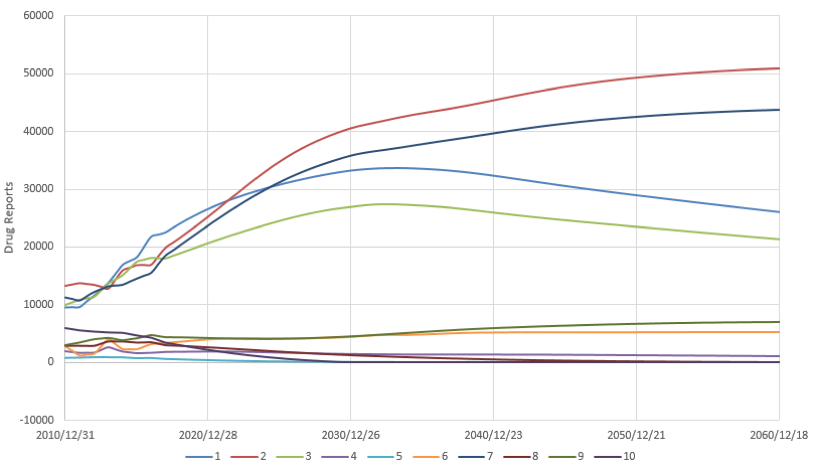
\includegraphics[scale=0.8]{./figures/12.png}
	\caption{}
	\label{Fig12}
\end{figure}

\section{Toward the Policy}
In this section, we will identify a possible strategy for countering the opioid crisis and use our model to test the effectiveness of this strategy. Before that, it’s necessary to have a close look at the historical policy to opioid users in the U.S.

\subsection{Historical Policies towards Opioid Users} %TODO: Reference
In U.S., the drug control started from 1940s, both use and sale of opioids are under supervision. Policicians were dedicated to enforce policies that impose penalties for drug users. Those users may feel pressure from every aspects, the government agencies, laws, and treatment programs\upcite{5}. We list major policies in the following paragraphs.

Some states started to limit needles and syringes for people without prescriptions from doctors ever since 1940s. To prevent heroin addiction, the needles/syringes possession was made a crime similar to heroin possession. This policy made herion addicts share needles with each other, which stimulated the increase of HIV and AIDS infection rate.

From late 1960s, the U.S. government started to treatment addicts with new medicine, particularly methadone maintenance treatment(MMT). It was proved that MMT was useful for drug users and decreased heroin use, and drug-related crimes were also reduced. The government also constructed communities for therapy, which supplied houses, abstinence-based recovery programs for people addicted to drugs\upcite{4}.

For those doesn't obey the drug control laws, police officers will impose sanctions accordingly. Public chose to take "Zero tolerance" attitude toward heroin users in view of heroin's harm. Therefore, both drug buyers and seller to took several measures to escape the inspection of the police. The sellers, made this activity unknown for as much people as they can, including neighbors, family members and even other heroin users\upcite{5}.

Because heroin and other opioids often have a high cost, it is normally not covered by the insurance, since the U.S. health system is mainly funded privately. And People who are jobless may face difficulties when using the income transfrom system, many drug users were even removed from the system in the 1990s. That means that they don't have stable income, job and even residence\upcite{5}.

Above all, the explanations of the current level which opioid use got to are various and complex. Some policies may have side effect, therefore the government should carefully select policy.

\subsection{Short-term Policy: Reducing the Natural Growth Rate of Major Domain}
In Section 4.2, we use the Lotka-Volterra equations to simulate the interactions between different clusters. This model prerequisite the environment is stable and thus not considering changes. So it is only suitable for short-term prediction. We utilize it to guide our short-term policy.

For each species-i, leaving out other sepcies' influence, it has a natural growth rate $a_{i}$ of itself, which is multipied by $\lambda$. Therefore, the first idea is to forcely decrease the $\lambda$ for regions. For instance, enforcing laws to penalize non-prescription use of drugs more strongly, from Fig. \ref{Fig14}, the dash line represents drug-use of restricting $a_{i}$, and the effect is significant.

\begin{figure}[H]
	\centering %图片全局居中
	%并排几个图,就要写几个minipage
	\begin{minipage}[b]{0.48\textwidth} %所有minipage宽度之和要小于1,否则会自动变成竖排
		\centering %图片局部居中
		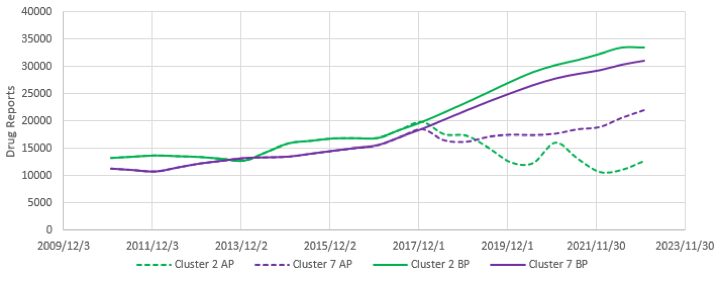
\includegraphics[scale=0.68]{./figures/13.png} %此时的图片宽度比例是相对于这个minipage的,不是全局
		% \caption{}
	\end{minipage}
	\begin{minipage}[b]{0.48\textwidth} %所有minipage宽度之和要小于1,否则会自动变成竖排
		\centering %图片局部居中
		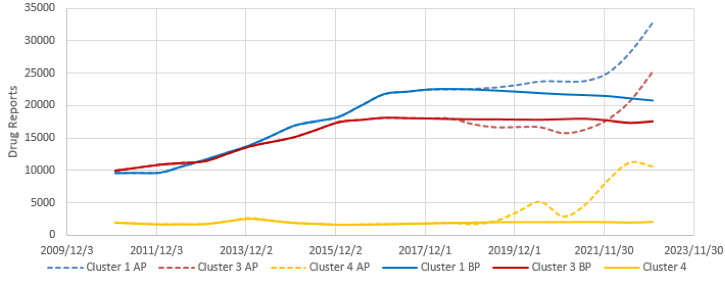
\includegraphics[scale=0.68]{./figures/14.png}%此时的图片宽度比例是相对于这个minipage的,不是全局
		% \caption{}
	\end{minipage}
	\caption{Drug Reports Change Before Policy(BP) and After Policy(AP) in Policy-Implemented Areas(left) and Other Areas(right)}
	\label{Fig14}
\end{figure}

However, Fig. \ref{Fig14} simultaneously demonstrates that when one area implements policies, adjacent areas without proper measures will face boom of drug-use crisis. This can be explained that people influenced in areas policy-implemented area will migrate there and more drugs may flow there after. Thereby, policies should be considered nationally, such as limiting opioids import, enforcing laws and more relevant policies. Fig. \ref{Fig16} proves the practicality.

\begin{figure}[H]
	\centering
	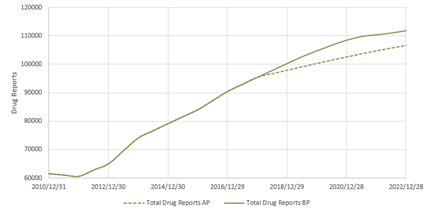
\includegraphics[scale=0.9]{./figures/16.png}
	\caption{Policies in an national scale}
	\label{Fig16}
\end{figure}

\subsection{Long-term Policy: Increasing Education Attainment and Married Rate}
Compared to the short-term policy, long-term policy could be some measures that influence the whole society and then regulate the drug-use level. In order to prove out view, we use the improved model to adjust the regional education factor and family factor (marriage rate, single female proportion and so on). When we change the value of above two factors by increasing them by 0.6 percentage, we obtain the dashed line presented in the Fig. \ref{Fig17}. It is clearly that these two factors can reduce the usage of drugs by more than 10\%, therefore we can believe that increasing the popularity of education, as well as encouraging marriage are conducive to affect and control the US drug-use level.
\begin{figure}[H]
	\centering
	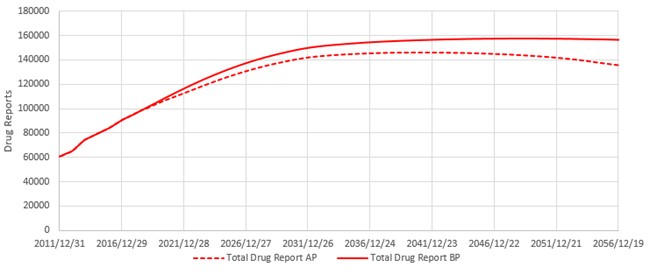
\includegraphics[scale=0.7]{./figures/17.png}
	\caption{Policies in the Long Term}
	\label{Fig17}
\end{figure}

\section{Strengths and Weaknesses}
\subsection{Strengths}
\begin{itemize}
	\item In the process of Drug Reports data, our model takes the idea of clustering, which overcomes the disadvantages of analyzing either the whole state or one single county. In the process of Census socio-economic data, we use the Entropy Weight Method to maximum compressed variables on the basis of maintaining certain economic logic.
	\item In order to identify where specific opioid use, we construct the Logistic Model for simplicity. And we get maximum number from the model to further determine threshold levels for caution. While forecasting its future patterns and characteristics, we ues and the Modified LVM to consider both the interaction and factors’ influence.
\end{itemize}

\subsection{Weaknesses}
\begin{itemize}
	\item Although we use the k-means clustering algorithm to replace five states into areas represented by ten clusters in order to simplify data processing, the subsequent analysis must be based on the clusters’ data. Therefore, it can not be accurately analyzed and that is to say here’s a certain error.
	\item Logistic regression model is suitable for most of the clusters data, but there are still 2 to 3 clusters which have decreasing trends. In the process of solving problems, we do not handle them by other models and also think that they will not exceed the threshold level. It seems kind of impractical.
 \end{itemize}

\begin{thebibliography}{99}
\addcontentsline{toc}{section}{References}  %引用部分标题("Refenrence")的重命名

\bibitem{1}MacQueen, J. (1967, June). Some methods for classification and analysis of multivariate observations. In Proceedings of the fifth Berkeley symposium on mathematical statistics and probability (Vol. 1, No. 14, pp. 281-297).
\bibitem{2}Gazetteer Files - Geography - U.S. Census Bureau. \texttt{\\https://www.census.gov/geo/maps-data/data/gazetteer.html}
\bibitem{3}Shannon, C. E. (1948). A mathematical theory of communication. Bell system technical journal, 27(3), 379-423.
\bibitem{4}DrugBank. \texttt{https://www.drugbank.ca/drug}
\bibitem{5}Johnson, B. D., Maher, L., \& Friedman, S. R. (2001). What public policies affect heroin users?. Journal of Applied Sociology, 14-49.
\bibitem{6}ZHANG Yu, GAO Kening, CHEN Mo, YU GA (2018). Method of Link Prediction Combining Network Structure and Node Attributes. Journal of Frontiers of Computer Science and Technology.
\bibitem{7}Carrieri, M. P., Amass, L., Lucas, G. M., Vlahov, D., Wodak, A., \& Woody, G. E. (2006). Buprenorphine use: the international experience. Clinical Infectious Diseases, 43(Supplement\_4), S197-S215.

\end{thebibliography}

\clearpage
\begin{appendices}
% \addcontentsline{toc}{section}{Appendix}  	% 将附录内容加入到目录中
\section{Figures}
\begin{figure}[H]
	\centering
	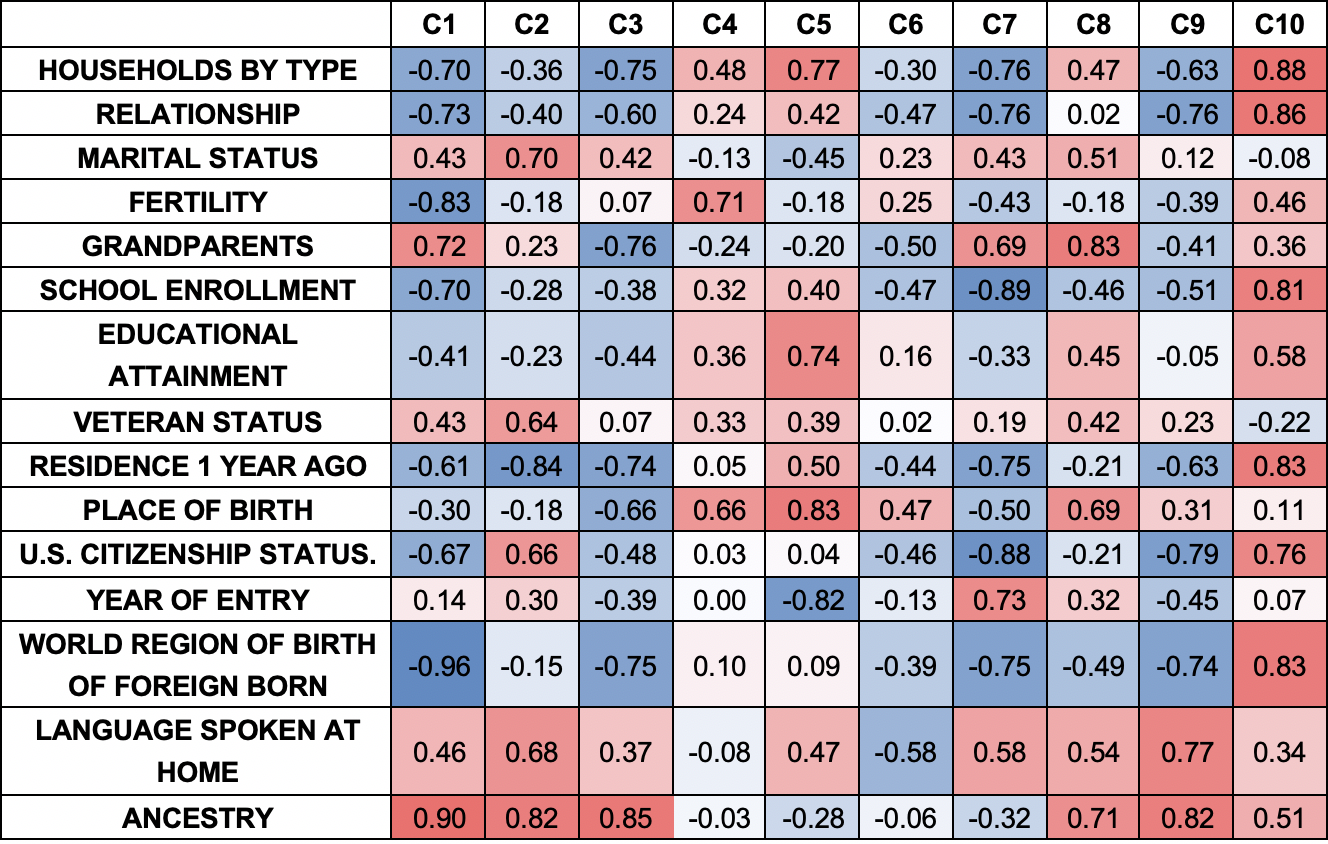
\includegraphics[scale=0.5]{./figures/a1.png}
	\caption{coefficients between Factors and Clusters}
\end{figure}

\section{The Source Codes}		% 附录标题可以自行修改


This python program implements k-means clustering.
\begin{lstlisting}[language={python}, caption=\texttt{k-means.py}]
from numpy import *
import time
from math import radians, cos, sin, asin, sqrt
import matplotlib.pyplot as plt
	

def calculate_dis(vec1,
					vec2):
	"""
	Calculate the distance between two places
	"""
	# print(vec1)
	# print(vec2)
	lat1 = vec1[0]
	lon1 = vec1[1]
	lat2 = vec2[0]
	lon2 = vec2[1]
	lon1, lat1, lon2, lat2 = map(radians, [lon1, lat1, lon2, lat2])
	
	# haversine
	dlon = lon2 - lon1 
	dlat = lat2 - lat1 
	a = sin(dlat/2)**2 + cos(lat1) * cos(lat2) * sin(dlon/2)**2
	c = 2 * asin(sqrt(a)) 
	r = 6371 # the radius of earth
	return c * r * 1000 # return in meters
	
# init centroids with random samples
def initCentroids(dataSet, k):
	numSamples, dim = dataSet.shape
	centroids = zeros((k, dim))
	for i in range(k):
		index = int(random.uniform(0, numSamples))
		centroids[i, :] = dataSet[index, :]
	return centroids
	
# k-means cluster
def kmeans(dataSet, k):
	numSamples = dataSet.shape[0]
	# first column stores which cluster this sample belongs to,
	# second column stores the error between this sample and its centroid
	clusterAssment = mat(zeros((numSamples, 2)))
	res = zeros((numSamples, 1))
	clusterChanged = True

	centroids = initCentroids(dataSet, k)

	while clusterChanged:
		clusterChanged = False
		## for each sample
		for i in range(numSamples):
			minDist  = 100000000000.0
			minIndex = 0
			## for each centroid
			## step 2: find the centroid who is closest
			for j in range(k):
				distance = calculate_dis(centroids[j, :], array(dataSet[i])[0]) #convert to array
				if distance < minDist:
					minDist  = distance
					# print("minDist", minDist)
					minIndex = j
					# print("minindex", minIndex)
			
			## step 3: update its cluster
			if clusterAssment[i, 0] != minIndex:
				clusterChanged = True
				clusterAssment[i, :] = minIndex, minDist**2
				res[i] = minIndex

		## step 4: update centroids
		for j in range(k):
			pointsInCluster = dataSet[nonzero(clusterAssment[:, 0].A == j)[0]]
			centroids[j, :] = mean(pointsInCluster, axis = 0)
	return centroids, clusterAssment, res
\end{lstlisting}
% \inputpython{../code/k-means.py}{0}{68}

This python program implements entropy weight method.
\begin{lstlisting}[language={python}, caption=\texttt{entropy-weight.py}]
import numpy as np
import pandas as pd

def entropy(dataset):
    n, k = np.shape(dataset)
    maximum = np.max(dataset, axis=0) #minimum in column
    minimum = np.min(dataset, axis=0)
    data = (dataset - minimum) * 1.0 / (maximum - minimum)
    col_sum = np.sum(data, axis=0)
    data = data / col_sum
    a = data * 1.0
    a[np.where(data==0)]=0.0001
    e = (-1.0/np.log(n))*np.sum(data*np.log(a), axis=0) # e 1*k
    w = (1 - e) / np.sum(1 - e)
    recodes = np.sum(dataset * w, axis=1)
    return recodes
\end{lstlisting}
% \lstinputlisting[language={python}, caption=\texttt{entropy\_weight.py}]{../code/entropy\_weight.py}

% This MATLAB program is used to calculate the value of variable $a$.
% \begin{lstlisting}[language={Matlab}, caption=\texttt{temp.m}]
% a = 0;
% for i = 1:5
% 	a = a + 1;
% end
% \end{lstlisting}

% This LINGO program is used to search the optimize solution of 0-1 problem.
% \begin{lstlisting}[language=Lingo, caption=\texttt{temp.lg4}]
% model:
% sets:
% WP/1..12/: M, W, X;
% endsets
% data:
% M = 2 5 18 3 2 5 10 4 11 7 14 6;
% W = 5 10 13 4 3 11 13 10 8 16 7 4;
% enddata
% max = @sum(WP:W*X);
% @sum(WP: M * X)<=46;
% @for(WP: @bin(X));
% end
% \end{lstlisting}

% \textbf{\textcolor[rgb]{0.98,0.00,0.00}{Input matlab source:}}
% % \lstinputlisting[language=Matlab]{../code/matlab-test.m}

\end{appendices}
\end{document}